
The general equation of a second degree can be expressed as :
\begin{align}
	\vec{x}^T\vec{V}\vec{x}+2\vec{u}^T\vec{x}+f=0\label{eq:solutions/4/2/7/gen__quad_eqn}
\end{align}
Let the equation of the tangent be
\begin{align}
	\myvec{-m & 1}\vec{x}=c \label{eq:solutions/4/2/7/given_line_eq}
\end{align}

We know that, for a circle, 
\begin{align}
	\vec{V} = \vec{I}  \\
	\vec{c} = -\vec{u}
\end{align}
Comparing the equation \eqref{eq:solutions/4/2/7/eq:1} and \eqref{eq:solutions/4/2/7/gen__quad_eqn}
we get
\begin{align}
	\vec{u}&=\myvec{-2 \\ -3}, f=12 \\
	\vec{c}&=\myvec{2 \\ 3}
\end{align} 

The normal vector to the line is obtained as 
\begin{align}
	\vec{n} = \vec{q} + \vec{u} \label{eq:solutions/4/2/7/eq1}\\
	\vec{q} = \vec{n} - \vec{u}
\end{align}

Comparing the equation \eqref{eq:solutions/4/2/7/given_line_eq} 
\begin{align}
	\vec{n} &= \myvec{-m &1}^T
\end{align}
Given
\begin{align}
	 \vec{u}&=\myvec{-2 \\ -3}\\
\implies	 \vec{q} &= \myvec{-m+2 \\ 4}\label{eq:solutions/4/2/7/eq:2}
\end{align}
The point q also satisfies the equation of the circle at \eqref{eq:solutions/4/2/7/gen__quad_eqn}
\begin{align}
	\vec{q}^T\vec{q}+2\vec{u}^T\vec{q}+f=0\\
	(\vec{n} -\vec{u})^T(\vec{n} -\vec{u})+2\vec{u}^T(\vec{n} -\vec{u}) +f =0\\
	\norm{\vec{n}}^2 - \vec{n}^T\vec{u}-\vec{u}^T\vec{n}+\norm{\vec{u}}^2+2\vec{u}^T\vec{n}- 2\norm{\vec{u}}^2+f=0\\
	\norm{\vec{n}}^2 -\norm{\vec{u}}^2+f=0\\
	m^2+1-13+12=0\\
	m^2=0\\
	m=0\label{eq:solutions/4/2/7/eq:3}
\end{align}
Simplying \eqref{eq:solutions/4/2/7/eq:3} and \eqref{eq:solutions/4/2/7/eq:2} we get
\begin{align}
	\vec{q} &= \myvec{2 \\ 4}
\end{align}

Let $\vec{p} =\myvec{7 \\ 4}$
The length of tangent is 
\begin{align}
	\norm{\vec{p}-\vec{q}}&= \sqrt{(7-2)^2 + (4-4)^2}\\
	&=\sqrt{25}\\
	&=5
\end{align}
\begin{figure}[!htbp]
 	\centering
 	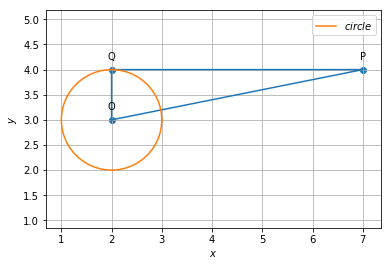
\includegraphics[width =\columnwidth]{./solutions/4/2/7/circle.png}
 	\caption{Perpendicular Line }
 	\label{eq:solutions/4/2/7/fig:1}
\end{figure}	

